\chapter{On ws-Continuous and ws-Irresolute Maps in Topological Spaces}
\ifpdf
  \graphicspath{{Chapter2/Chapter2Figs/}}
\else
\graphicspath{{Chapter2/Chapter2Figs/EPS/}{Chapter2/Chapter2Figs/}}
\fi

\parindent 0.75cm
\parskip 0.25cm

\newtheorem{theorem}{Theorem}[section]
\theoremstyle{plain}
\newtheorem{acknowledgement}{Acknowledgement}
\newtheorem{algorithm}{Algorithm}[section]
\newtheorem{axiom}{Axiom}[section]
\newtheorem{case}{Case}[section]
\newtheorem{claim}{Claim}[section]
\newtheorem{conclusion}{Conclusion}[section]
\newtheorem{condition}{Condition}[section]
\newtheorem{conjecture}{Conjecture}[section]
\newtheorem{corollary}[theorem]{Corollary}
\newtheorem{criterion}{Criterion}[section]
\newtheorem{definition}{Definition}[section]
\newtheorem{example}{Example}[section]
\newtheorem{exercise}{Exercise}[section]
\newtheorem{lemma}{Lemma}[section]
\newtheorem{notation}{Notation}[section]
\newtheorem{problem}{Problem}[section]
\newtheorem{proposition}{Proposition}[section]
\newtheorem{remark}[theorem]{Remark}
\newtheorem{solution}{Solution}[section]
\newtheorem{summary}{Summary}[section]
\numberwithin{equation}{section}
\def\baselinestretch{1.5}

%
Hand-drawn figures, downloaded/created images \& graphs need to be inserted in a document. There are different ways to insert these in a document. 


\section{Insert an image}

One image as in Figure \ref{Fig21} is to be inserted. Looks good if it is located in the center. The size can be adjusted to suit the needs. 

\begin{figure}[!htbp]
  \begin{center}
    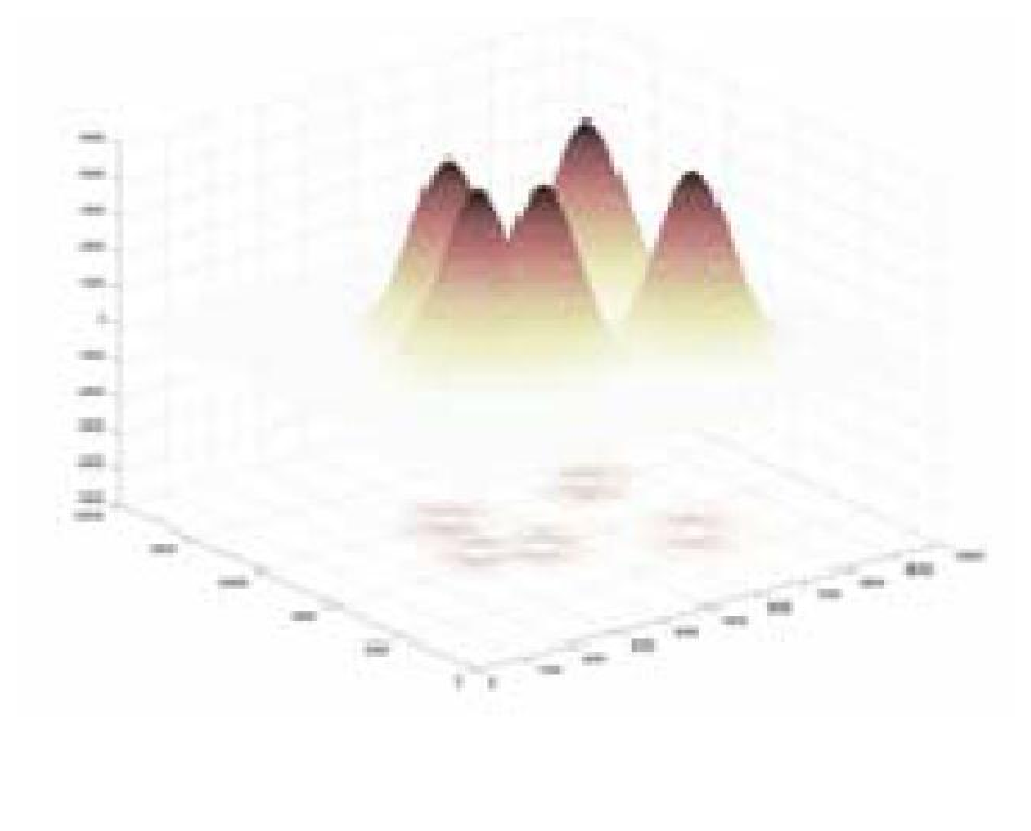
\includegraphics [scale=0.5]{small_width}
    \caption{Gaussian kernel}
    \label{Fig21}
  \end{center}
\end{figure}

\section{introduction}
The concept of continuous functions plays a very important role in general topology. The regular continuous and completely continuous functions are introduced and studied by Arya S P [2]. Later, R S wali et all [31] introduced and investigated αrw-continuous functions in topological spaces. 
Second part of this chapter, a new class of maps called weakly semi closed-continuous (briefly, ws-continuous) maps are introduced and analyzed their properties with other existing generalized continuous maps.
Third part of this chapter, we analyse the concepts of ws-irresolute maps and strongly ws-continuous maps in topological spaces and investigate some of their properties.
\section{ws-continuous maps and some of their properties.}
\definition{}